\section{Results}
\label{sec:results}
\subsection{RQ1: Localization with the Full Denominator}
Table~\ref{tab:means} reports S0 and S1 separately. S1 FR@5 is \SOneAgentFR{} for Agent, \SOneRagFR{} for RAG, and \SOnePackFR{} for Pack. The primary Agent--Pack difference is \SOnePrimary{}, with 95\% entry-bootstrap interval \SOnePrimaryCI{} and Monte Carlo $p=1/100001$. RAG--Pack FR@5 differs by 0.3500. Both query-dependent configurations exceed the lexical-prefix reference on this sample.
% Generated by paper/generate_revision_artifacts.py; see paper/provenance.json
\begin{table}[t]
\centering
\caption{File and line localization in the two studies. Each cell averages three repeats within each of 80 entries; all failures remain in the denominator.}\label{tab:means}
\small
\begin{adjustbox}{max width=\columnwidth}\begin{tabular}{llrrr}
\toprule
Study & Configuration & FR@5 & LR@5 & Failures \\
\midrule
S0 & Agent & 0.8458 & 0.6583 & 6/240 \\
S0 & RAG & 0.7875 & 0.4917 & 0/240 \\
S0 & Pack & 0.4271 & 0.2375 & 0/240 \\
S1 & Agent & 0.7479 & 0.5813 & 31/240 \\
S1 & RAG & 0.7729 & 0.4938 & 0/240 \\
S1 & Pack & 0.4229 & 0.2500 & 0/240 \\
\bottomrule
\end{tabular}\end{adjustbox}
\par\vspace{3pt}\begin{minipage}{\columnwidth}\footnotesize S0: original configuration study. S1: supplementary study on the same known sample, with a common eligible source universe and native Agent tools. These are separate studies, not independent samples.\end{minipage}
\end{table}

% Generated by paper/generate_revision_artifacts.py; see paper/provenance.json
\begin{table*}[t]
\centering
\caption{S1 paired comparisons using the frozen analysis. Differences use the first configuration minus the second.}\label{tab:contrasts}
\small
\begin{adjustbox}{max width=\textwidth}\begin{tabular}{llrrll}
\toprule
Comparison & Role & $\Delta$ & 95\% entry-bootstrap CI & $p$ & BH $q$ \\
\midrule
Agent--Pack FR & Primary & 0.3250 & [0.2271, 0.4229] & $<0.0001$ & --- \\
Agent--RAG FR & Secondary & -0.0250 & [-0.0771, 0.0271] & 0.3970 & 0.3970 \\
Agent--RAG LR & Secondary & 0.0875 & [0.0250, 0.1521] & 0.0112 & 0.0149 \\
RAG--Pack FR & Secondary & 0.3500 & [0.2583, 0.4396] & $<0.0001$ & $<0.0001$ \\
RAG--Pack LR & Secondary & 0.2438 & [0.1604, 0.3271] & $<0.0001$ & $<0.0001$ \\
\bottomrule
\end{tabular}\end{adjustbox}
\par\vspace{3pt}\begin{minipage}{\textwidth}\footnotesize Two-sided Monte Carlo sign flips: 100,000 draws, plus-one correction. The four secondary comparisons form one BH family with the frozen threshold $q<0.10$. Intervals resample entries and are not adjusted for repository clustering or multiple comparisons.\end{minipage}
\end{table*}


The Agent--RAG file contrast is \SOneAgentRagFR{}, with interval [-0.0771, 0.0271] and $p=q=\SOneAgentRagFRP{}$. It does not meet the frozen secondary criterion. The interval allows an Agent disadvantage of 7.71 percentage points and an advantage of 2.71 points under the entry-resampling assumptions; this result does not establish equivalence. Agent--RAG LR@5 differs by \SOneAgentRagLR{}, with interval [0.0250, 0.1521] and BH $q=\SOneAgentRagLRQ{}$ under the same entry-independence assumption. RAG--Pack LR@5 differs by 0.2438 (Table~\ref{tab:contrasts}).

Table~\ref{tab:cluster-sensitivity} places these contrasts alongside the post hoc repository diagnostics. For Agent--RAG LR@5, the equal-repository mean is 0.0533, and the exact repository sign-flip probability is 0.0781, with exploratory secondary $q=0.1042$. Thus the observed 0.0875 entry-weighted difference remains a sample description, while secondary inferential support is sensitive to the dependence assumptions. RAG--Pack FR@5 also has exploratory repository $q=0.1042$, compared with 0.0059 for RAG--Pack LR@5. These probabilities are separate sensitivities, not replacements for the frozen analysis or proof of general repository-level effects.
% Generated by paper/generate_review_sensitivity.py; see review_sensitivity_provenance.json
\begin{table*}[t]
\centering\small
\caption{Post-hoc S1 repository sensitivity for all frozen contrasts.}\label{tab:cluster-sensitivity}
\begin{adjustbox}{max width=\textwidth}\begin{tabular}{lrrrrr}
\toprule
Contrast & Entry mean & Equal-repo mean & Leave-one-repo range & Repo $p$ & Repo $q$ \\
\midrule
Agent--Pack FR & 0.3250 & 0.2228 & [0.2894, 0.3377] & 0.0313 & --- \\
Agent--RAG FR & -0.0250 & 0.0209 & [-0.0463, 0.0049] & 0.6250 & 0.6250 \\
RAG--Pack FR & 0.3500 & 0.2018 & [0.3186, 0.3701] & 0.0625 & 0.1042 \\
Agent--RAG LR & 0.0875 & 0.0533 & [0.0787, 0.0952] & 0.0781 & 0.1042 \\
RAG--Pack LR & 0.2438 & 0.3943 & [0.2245, 0.3238] & 0.0015 & 0.0059 \\
\bottomrule
\end{tabular}\end{adjustbox}
\par\vspace{3pt}\begin{minipage}{\textwidth}\footnotesize Repeats are averaged within entries before grouping the 80 entries into 13 repositories. Exact two-sided sign flips enumerate all $2^{13}=8{,}192$ repository signs using sums of entry differences; this retains the entry-weighted estimand and assumes independently sign-exchangeable repository contributions. The last column is exploratory Benjamini--Hochberg correction across the four secondary comparisons. It does not replace frozen entry-level inference or provide general cluster-robust validity. Equal-repository means target a different weighting.\end{minipage}
\end{table*}


\begin{figure}[t]
\centering
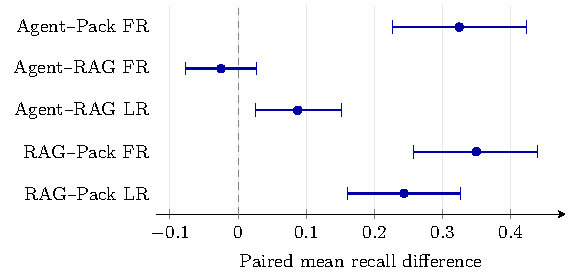
\includegraphics[width=\columnwidth]{figures/s1_contrasts.pdf}
\caption{S1 paired mean differences and 95\% entry-bootstrap intervals from the frozen analysis. FR is file coverage; LR is tolerance-based interval recall. Intervals are unadjusted and assume independent entries.}
\label{fig:contrasts}
\end{figure}

S0's Agent--Pack FR@5 difference is 0.4188, with interval [0.3333, 0.5062]. Its Agent--RAG file contrast is positive, 0.0583, with $p=q=0.0529$ under S0's secondary procedure. The latter passes S0's frozen $q<0.10$ criterion but not a per-comparison $p<0.05$ threshold. In S1 the point estimate changes sign. These observations accompany the bundled configuration changes; they are not evidence that a particular repair caused the difference.

\subsection{RQ2: Evidence Delivery and Final Output}
Table~\ref{tab:delivery} separates source acquisition from prediction. Agent delivers code from 48.0 unique paths per unit on average, RAG 51.5, and Pack 51.7. Their mean fractions of target files with any delivered source are 0.9542, 0.6813, and 0.0000. The fractions average each unit's one- or two-file target coverage; they are not pooled counts across three repeats.
% Generated by paper/generate_revision_artifacts.py; see paper/provenance.json
\begin{table}[t]
\centering
\caption{S1 descriptive context delivery and supplementary line scoring. Source files count unique paths with delivered code spans; directory and path-only listings are excluded.}\label{tab:delivery}
\small
\begin{adjustbox}{max width=\columnwidth}\begin{tabular}{lrrr}
\toprule
Configuration & Files/unit & Mean $|T\cap F(S)|/|T|$ & LR@5$_{\leq64}$ \\
\midrule
Agent & 48.0 & 0.9542 & 0.5042 \\
RAG & 51.5 & 0.6813 & 0.2729 \\
Pack & 51.7 & 0.0000 & 0.0208 \\
\bottomrule
\end{tabular}\end{adjustbox}
\par\vspace{3pt}\begin{minipage}{\columnwidth}\footnotesize Target fractions are averaged per unit, with one or two EP/CO target files per entry. The last column excludes predicted intervals longer than 64 lines; it remains an overlap-based recall measure.\end{minipage}
\end{table}


Agent's higher delivery coverage coexists with lower aggregate FR@5 than RAG. A hit in a target file can expose irrelevant lines, and a final prediction can omit an acquired target. The present summaries establish this difference between availability and output, without isolating those explanations. Pack achieves FR@5 \SOnePackFR{} despite no target-source delivery. The model still receives the advisory and path list; these and prior knowledge are possible information routes, whose individual contributions are not measured.

\subsection{Annotated Source, Returned Locations, and Prediction Extent}
The post hoc joint analysis moves from any code in a target file to overlap with its annotated interval. Mean annotation-source delivery is 0.9125 for Agent, 0.3813 for RAG, and zero for Pack, retaining all outcomes. Table~\ref{tab:annotation-stages} partitions 480 opportunities per arm. Agent has 279 credited interval hits, all accompanied by delivered annotation source. It also leaves 108 annotations uncovered in schema-valid outputs with such source available. RAG has 141 hits with annotation source and 96 without it; its uncovered annotations in schema-valid outputs divide into 102 without target-file code, 99 with only other lines from that file, and 42 with annotation-source delivery. Pack's 120 hits all occur without target-file source. Source and hit co-occurrence is an availability diagnostic; reasons and security traces are not adjudicated.
% Generated by generate_input_output_diagnostics.py; see input_output_provenance.json
\begin{table*}[t]
\centering\small
\caption{Joint annotation-level source and output outcomes in S1 (post hoc).}\label{tab:annotation-stages}
\begin{adjustbox}{max width=\textwidth}\begin{tabular}{lrrrrrr}
\toprule
Configuration & Invalid & Hit + source & Hit, no source & Miss, no file & Miss, file only & Miss + source \\
\midrule
Agent & 62 & 279 & 0 & 14 & 17 & 108 \\
RAG & 0 & 141 & 96 & 102 & 99 & 42 \\
Pack & 0 & 0 & 120 & 360 & 0 & 0 \\
\bottomrule
\end{tabular}\end{adjustbox}
\par\vspace{3pt}\begin{minipage}{\textwidth}\footnotesize Each row partitions all 480 EP/CO opportunities (240 outcomes, two annotations each). Source means exact overlap of delivered code with the annotated interval; a hit uses the frozen five-line-tolerance rule. Invalid output overrides source categories. Hit/source co-occurrence does not verify model use or rationale.\end{minipage}
\end{table*}

% Generated by generate_input_output_diagnostics.py; see input_output_provenance.json
\begin{table*}[t]
\centering\small
\caption{Annotation delivery, role recall, and predicted interval extent (post hoc).}\label{tab:interval-detail}
\begin{adjustbox}{max width=\textwidth}\begin{tabular}{lrrrrrr}
\toprule
Configuration & Annotation source & EP recall & CO recall & Width median & Width P90 & Union lines/unit \\
\midrule
Agent & 0.9125 & 0.4083 & 0.7542 & 22.0 & 75.0 & 88.4 \\
RAG & 0.3813 & 0.3750 & 0.6125 & 38.0 & 220.0 & 264.9 \\
Pack & 0.0000 & 0.2375 & 0.2625 & 200.0 & 300.0 & 629.8 \\
\bottomrule
\end{tabular}\end{adjustbox}
\par\vspace{3pt}\begin{minipage}{\textwidth}\footnotesize Annotation source is averaged over all 480 annotation opportunities. EP and CO recall each retain 240 outcomes. Width quantiles summarize intervals in valid top-five answers; union lines/unit merges overlapping predicted intervals within a file and averages all 240 outcomes, including zero lines for failures. These are model-reported numeric extents, including absent paths and out-of-bounds lines, not readable code or measured human effort.\end{minipage}
\end{table*}


% Generated by generate_review_resolution.py; see review_resolution_provenance.json
\begin{table*}[t]
\centering\small
\caption{Joint annotation coverage by role and prediction width (post hoc).}\label{tab:role-width}
\begin{adjustbox}{max width=\textwidth}\begin{tabular}{lrrrrrr}
\toprule
Configuration & Role & Source, no hit & Correct path subset & Hit, no ann. source & Retained at 64 & No file source subset \\
\midrule
Agent & EP & 80 & 53 & 0 & 0 & 0 \\
Agent & CO & 28 & 25 & 0 & 0 & 0 \\
RAG & EP & 36 & 23 & 39 & 0 & 26 \\
RAG & CO & 6 & 3 & 57 & 5 & 25 \\
Pack & EP & 0 & 0 & 57 & 4 & 57 \\
Pack & CO & 0 & 0 & 63 & 6 & 63 \\
\bottomrule
\end{tabular}\end{adjustbox}
\par\vspace{3pt}\begin{minipage}{\textwidth}\footnotesize Each role has 240 opportunities. Source/no-hit requires schema-valid output; the next column is its correct-path subset. The final two columns are subsets of hits without annotated source. Retained at 64 uses the frozen width-limited rule. Categories describe co-occurrence, not task failure or evidence use.\end{minipage}
\end{table*}

% Generated by generate_review_resolution.py; see review_resolution_provenance.json
\begin{table*}[t]
\centering\small
\caption{Repository validity of returned intervals (post hoc).}\label{tab:location-validity}
\begin{adjustbox}{max width=\textwidth}\begin{tabular}{lrrrrr}
\toprule
Configuration & Intervals & Absent path & End beyond EOF & Affected units / 240 & Clipped lines/unit \\
\midrule
Agent & 635 & 0 & 2 & 2 & 88.2 \\
RAG & 774 & 23 & 52 & 56 & 228.8 \\
Pack & 763 & 381 & 129 & 180 & 261.5 \\
\bottomrule
\end{tabular}\end{adjustbox}
\par\vspace{3pt}\begin{minipage}{\textwidth}\footnotesize Counts refer to top-five predictions. Paths are checked against the complete pinned Git tree; existing files use recorded line counts. Three Pack intervals refer to existing filtered files. Clipped extent drops absent paths, bounds intervals by file length, merges within each path, and averages all 240 outcomes including failures. These diagnostics do not rescore frozen outcomes or measure analyst effort.\end{minipage}
\end{table*}


Table~\ref{tab:role-width} clarifies the coverage categories. Of Agent's 108 uncovered annotations with source available, 80 are EP and 28 CO; 78 already have the correct file among the predictions. Two purposively selected counterexamples illustrate why this is not automatically task failure. For \texttt{entry-00227}, repeat 1, Agent returns lines 121--146 of \path{src/agents/tools/sessions-spawn-tool.ts}, covering the CO at line 129 but not the EP factory declaration at line 60. For \texttt{entry-00229}, repeat 1, its lines 253--267 of \path{src/agents/apply-patch.ts} cover the sandbox operation at CO line 258, not the EP factory at line 80. These cases demonstrate role-specific annotation omissions while a critical operation is returned; they do not validate every rationale or estimate their prevalence.

Of RAG's 96 hits without corresponding annotation source, 45 have other source from the target file and 51 have none. Only five retain a hit under the 64-line rule, all at CO; the other 91 depend on broader returned intervals. Pack retains ten of its 120 such hits. Thus hits without annotated source predominantly describe broad overlap credit in these records, rather than demonstrated precise localization without source.

Table~\ref{tab:location-validity} separates schema acceptance from repository-valid locations. RAG's 774 returned intervals contain 23 nonexistent paths and 52 intervals ending beyond the file; Pack's 763 contain 381 and 129 respectively. Agent's 635 contain no nonexistent paths and two overruns. At least one such issue occurs in 56 RAG, 180 Pack, and two Agent outcomes. For example, Pack predicts lines 1--250 of \path{packages/server/src/routes/chatflows/index.ts} in \texttt{entry-00477}, whose file contains 43 lines. After removing absent paths and clipping to file lengths, mean within-file union extents are 88.2, 228.8, and 261.5 lines per outcome for Agent, RAG, and Pack. These are descriptive location checks, not replacements for the frozen scores.


Prediction extents help interpret those hits. Across returned top-five intervals, median widths are 22 lines for Agent, 38 for RAG, and 200 for Pack; the corresponding 90th percentiles are 75, 220, and 300. Mean within-file union extents per scheduled outcome are 88.4, 264.9, and 629.8 lines, including zero for failures. These are model-reported numeric extents, including nonexistent paths and out-of-bounds lines; they do not measure readable source or analyst effort. Agent's EP and CO recalls are 0.4083 and 0.7542, versus RAG's 0.3750 and 0.6125: the larger role-specific difference is at CO.

Width-limited LR@5$_{\leq64}$ is 0.5042 for Agent, 0.2729 for RAG, and 0.0208 for Pack. Relative to ordinary LR@5, excluding broad intervals reduces Agent's score by 0.0771, RAG's by 0.2208, and Pack's by 0.2292. The difference between the line measures is consequential, especially for RAG and Pack. Agent's higher width-limited point estimate remains descriptive; no additional significance test was registered.

S1 retains 31 Agent output failures: 22 final DSML tool-call texts and nine empty final text fields. The nine empty fields arise from completed assistant messages containing thinking but no text, rather than absence of any assistant message. RAG and Pack have no schema-level output failures; location-validity issues are counted separately. All 31 Agent failures contribute zeros to the reported means.

A descriptive paired decomposition retains the denominator of 240: Agent's 209 valid-output units contribute $+0.0521$ to Agent--RAG FR@5, while its 31 invalid-output units contribute $-0.0771$, summing to $-0.0250$. For LR@5, the contributions are $+0.1229$ and $-0.0354$, summing to $+0.0875$. These are contributions to the observed contrast, not subset performance estimates or a forecast for a repaired Agent.

The native events locate an operational boundary (Table~\ref{tab:completion}). Active tools close in 53 Agent units: 36 reach 40 accepted bridge actions and 17 exhaust the information budget. Those units include 22 valid answers and all 31 failures; the other 187 units return valid answers. All 22 DSML failures receive an explicit final-JSON formatting correction and remain invalid. The nine empty outputs receive no correction. Only one failed unit receives the bridge's fixed budget-exhausted text.
% Generated by paper/generate_revision_artifacts.py; see paper/provenance.json
\begin{table}[t]
\centering
\caption{S1 Agent final-output status by observed tool-declaration closure (post-hoc).}\label{tab:completion}
\small
\begin{adjustbox}{max width=\columnwidth}\begin{tabular}{lrrrr}
\toprule
Tool state & Units & Schema-valid & DSML & Empty \\
\midrule
Never closed & 187 & 187 & 0 & 0 \\
Closed & 53 & 22 & 22 & 9 \\
\bottomrule
\end{tabular}\end{adjustbox}
\par\vspace{3pt}\begin{minipage}{\columnwidth}\footnotesize Closure follows the information or accepted-action limit. DSML denotes terminal tool-call text outside the allowed final-answer protocol. All failed units score zero. Groups are selected by an observed outcome of execution, not randomized treatments.\end{minipage}
\end{table}


\begin{figure}[t]
\centering
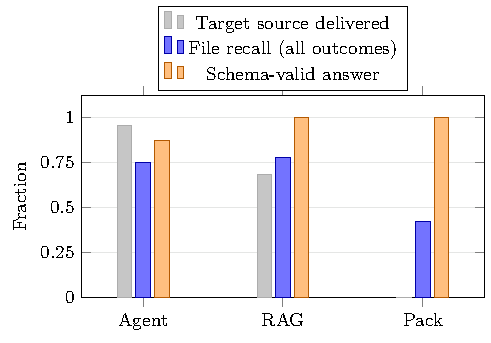
\includegraphics[width=\columnwidth]{figures/s1_delivery_output.pdf}
\caption{S1 mean target-file source coverage, FR@5, and schema-valid answer fractions across all 240 outcomes per configuration. Schema acceptance does not certify path existence, line bounds, or location correctness.}
\label{fig:delivery-output}
\end{figure}

Reviewing all saved native completion events finds no earlier usable final localization JSON overwritten in the 31 failures. Their final texts are also unrecoverable by S0's permissive parser. These observations support retaining the output failures; they do not establish that the shutdown behavior alone caused them.

\subsection{RQ3: Resources and Online Time}
Table~\ref{tab:resources} includes all 240 effective outcomes per arm, including failures. Agent's mean ledger count is 31,376 tokens, compared with approximately 50,000 for RAG and Pack. Its cumulative provider input averages 572,748 tokens, against 53,637 for RAG and 54,194 for Pack. Thus Agent uses fewer newly acquired ledger tokens but \SOneInputRatio{} times Pack's provider input. The shared acquisition ceiling does not equalize model work.
% Generated by paper/generate_revision_artifacts.py; see paper/provenance.json
\begin{table*}[t]
\centering
\caption{S1 measured resources for 240 outcomes per configuration, including model-output failures. Fees cover effective outcomes; superseded attempts are reported separately.}\label{tab:resources}
\small
\begin{adjustbox}{max width=\textwidth}\begin{tabular}{lrrrrr}
\toprule
Configuration & Mean $A$ & Mean $B$ & Fee (USD) & Mean time (s) & Median time (s) \\
\midrule
Agent & 31,376 & 572,748 & 27.154 & 107.9 & 102.8 \\
RAG & 49,996 & 53,637 & 10.120 & 58.2 & 52.9 \\
Pack & 49,994 & 54,194 & 9.970 & 52.9 & 47.2 \\
\bottomrule
\end{tabular}\end{adjustbox}
\par\vspace{3pt}\begin{minipage}{\textwidth}\footnotesize $A$: newly delivered blocks in the accounting tokenizer. $B$: cumulative provider input, including replayed history and cached input. Unit time starts after initial source/index checks and some model preparation; offline index construction and failed infrastructure attempts are outside this measure.\end{minipage}
\end{table*}


\begin{figure}[t]
\centering
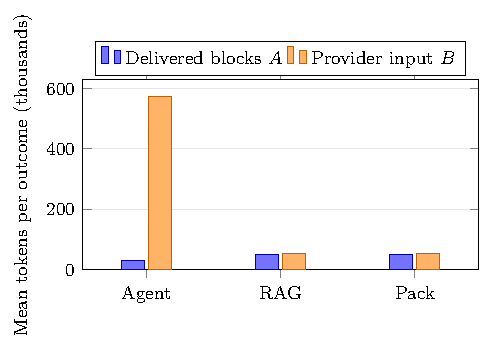
\includegraphics[width=\columnwidth]{figures/s1_input.pdf}
\caption{S1 descriptive means for newly delivered ledger information $A$ and cumulative provider input $B$. Their tokenizer and scope differ; the plot does not compare interchangeable budgets.}
\label{fig:input}
\end{figure}

Effective-outcome fees total USD \SOneFee{}. Including reported superseded attempts yields a known subtotal of USD \SOneAllFee{}, plus two historical requests whose charges remain unknown. Development calls, local compute, and index preparation are outside this subtotal. Fees are usage reports rather than independently reconciled supplier invoices.

Mean recorded unit times are 107.9 seconds for Agent, 58.2 for RAG, and 52.9 for Pack; medians are 102.8, 52.9, and 47.2 seconds. These describe the measured execution window and observed service conditions. Offline indexing is a separate investment, and initial validation/loading outside the window prevents interpreting these values as full end-to-end deployment latency.

\subsection{Sample Composition Sensitivity}
Removing any one repository leaves a positive S1 Agent--Pack aggregate contrast, ranging from \SOneLocoMin{} to \SOneLocoMax{}. The equal-repository mean is \SOneRepoEqual{}, compared with the entry-weighted \SOnePrimary{}. The frozen repository-resampling interval is [0.1500, 0.4363]. Per-repository contrasts include negatives for WeKnora and Airflow and zeros for several projects (Appendix~B). These small groups and unequal weights limit precision and generality despite a positive overall contrast. Leave-out stability does not validate the entry-independence assumption.

Table~\ref{tab:hint-subgroups} describes all S1 outcomes within the 29 description-hint and 51 description-no-match entries. Each arm has 87 and 153 outcomes respectively; Agent's four and 27 failures remain scored zero. File recall is higher in the description-hint stratum for every configuration. Pack's means are 0.7241 and 0.2516, despite no target-source delivery in either stratum. These strata differ in task and repository composition, and the latter still includes 35 titles matching target basenames. Their score difference describes the frozen description flags rather than the effect of input hints.
% Generated by paper/generate_review_sensitivity.py; see review_sensitivity_provenance.json
\begin{table*}[t]
\centering\small
\caption{S1 descriptive outcomes by the frozen description-only hint flag.}\label{tab:hint-subgroups}
\begin{adjustbox}{max width=\textwidth}\begin{tabular}{lrlrrr}
\toprule
Advisory label & Entries & Configuration & FR@5 & LR@5 & Failed \\
\midrule
PATH\_HINT & 29 & Agent & 0.8448 & 0.6034 & 4/87 \\
PATH\_HINT & 29 & RAG & 0.8621 & 0.6207 & 0/87 \\
PATH\_HINT & 29 & Pack & 0.7241 & 0.4080 & 0/87 \\
NO\_PATH\_HINT & 51 & Agent & 0.6928 & 0.5686 & 27/153 \\
NO\_PATH\_HINT & 51 & RAG & 0.7222 & 0.4216 & 0/153 \\
NO\_PATH\_HINT & 51 & Pack & 0.2516 & 0.1601 & 0/153 \\
\bottomrule
\end{tabular}\end{adjustbox}
\par\vspace{3pt}\begin{minipage}{\textwidth}\footnotesize All outcomes, including failed final answers, remain in each subgroup denominator. Labels are from the original frozen annotation rule. This is an observational subgroup description without new significance tests, a masking intervention, or contamination detection.\end{minipage}
\end{table*}


For an input-provenance example, \texttt{entry-00383} is the first evaluated entry in the frozen manifest. Its dataset title ends in \texttt{request-policy.ts}, matching target \path{src/browser/request-policy.ts}; the original title of \href{https://github.com/advisories/GHSA-xp9r-prpg-373r}{GHSA-XP9R-PRPG-373R} has no filename suffix. Its truncated description is flagged \texttt{NO\_PATH\_HINT}. This title reached all three configurations, illustrating why the description-only label cannot identify a hint-free task. Selection follows manifest order rather than scores.
